% !TEX TS-program = pdflatex
% !TEX encoding = UTF-8 Unicode

% This is a simple template for a LaTeX document using the "article" class.
% See "book", "report", "letter" for other types of document.

\documentclass[11pt]{article} % use larger type; default would be 10pt

\usepackage{amsmath,amssymb}
\usepackage[utf8]{inputenc} % set input encoding (not needed with XeLaTeX)

%%% Examples of Article customizations
% These packages are optional, depending whether you want the features they provide.
% See the LaTeX Companion or other references for full information.

%%% PAGE 
\usepackage{geometry} % to change the page dimensions
\geometry{letterpaper} % or letterpaper (US) or a5paper or....
% \geometry{margin=2in} % for example, change the margins to 2 inches all round
% \geometry{landscape} % set up the page for landscape
%   read geometry.pdf for detailed page layout information

\usepackage{graphicx} % support the \includegraphics command and options

% \usepackage[parfill]{parskip} % Activate to begin paragraphs with an empty line rather than an indent

%%% PACKAGES
\usepackage{booktabs} % for much better looking tables
\usepackage{array} % for better arrays (eg matrices) in maths
\usepackage{paralist} % very flexible & customisable lists (eg. enumerate/itemize, etc.)
\usepackage{verbatim} % adds environment for commenting out blocks of text & for better verbatim
\usepackage{subfig} % make it possible to include more than one captioned figure/table in a single float
% These packages are all incorporated in the memoir class to one degree or another...

%%% HEADERS & FOOTERS
\usepackage{fancyhdr} % This should be set AFTER setting up the page geometry
\pagestyle{fancy} % options: empty , plain , fancy
\renewcommand{\headrulewidth}{0pt} % customise the layout...
\lhead{}\chead{}\rhead{}
\lfoot{}\cfoot{\thepage}\rfoot{}

%%% SECTION TITLE APPEARANCE
\usepackage{sectsty}
\allsectionsfont{\sffamily\mdseries\upshape} % (See the fntguide.pdf for font help)
% (This matches ConTeXt defaults)

%%% ToC (table of contents) APPEARANCE
\usepackage[nottoc,notlof,notlot]{tocbibind} % Put the bibliography in the ToC
\usepackage[titles,subfigure]{tocloft} % Alter the style of the Table of Contents
\renewcommand{\cftsecfont}{\rmfamily\mdseries\upshape}
\renewcommand{\cftsecpagefont}{\rmfamily\mdseries\upshape} % No bold!

%%% END Article customizations

%%% The "real" document content comes below...

\title{Consequences of Pauli blocking between paired fermions on Feshbach resonances}
%\author{The Author}
%\date{} % Activate to display a given date or no date (if empty),
         % otherwise the current date is printed 
\input{../newcommand}
\begin{document}
\maketitle

\section{Model system}

We consider a system made of two different fermionic atoms, $\alpha$ and $\beta$.  These fermions can be in two coupled subbands. Let $\alpha^{\dg}_{\vk, \nu}$ and $\beta^{\dg}_{\vk,\nu}$, be the creation operators of fermions $\alpha$ and $\beta$ with momentum $\vk$ in one of their two subbands, $\nu=\pm1$. 

The Hamiltonian f this two-atom system reads as 
\begin{equation}
\mathcal{H}=\mathcal{H}_0+\mathcal{V}
\end{equation}
$\mathcal{H}_0$ is e free fermionic kinetic energy. 	
\begin{equation}
\mathcal{H}_0=\sum_{\nu=\pm1}\sum_{\vk}{(\epsilon_{\mathbf{k}}+\delta^{(\alpha)}_{\nu})\alpha^{\dg}_{\vk, \nu}\alpha^{}_{\vk, \nu}
+(\epsilon_{\mathbf{k}}+\delta^{(\beta)}_{\nu})\beta^{\dg}_{\vk, \nu}\beta^{}_{\vk, \nu}}				
\end{equation}	
where $\epsilon_{\mathbf{k}}=k^2/2m$ if these two atoms are taken with the same mass.  The lowest energy of the two $\alpha$ and $\beta$ subbands are $\eta_{\nu}^{(\alpha)}$ and 	 $\eta_{\nu}^{(\beta)}$ respectively. 

These $(\alpha,\beta)$ fermions are assumed to interact through a BCS-like separable potential having diagonal and non-diagonal processes.  This interaction potential, shown with 1, can be written as 
\begin{equation}
\mathcal{V}=-\sum_{\{\nu\}}\sum_{\vk\vk'}w_{\vk}w_{\vk'}V 
\begin{pmatrix}
\nu_{\alpha}^{'}&\nu_{\alpha}^{}\\
\nu_{\beta}^{'}&\nu_{\beta}^{}
\end{pmatrix}
B^{\dg}_{\mathbf{k}^{'},\nu_{\alpha}^{'},\nu_{\beta}^{'}}
B^{\dg}_{\mathbf{k}^{ },\nu_{\alpha}^{},\nu_{\beta}^{}}
\end{equation}
where, in order for $\mathcal{V}$ to be equal  $\mathcal{V}^{\dg}$, the $V 
\left(\begin{smallmatrix}
\nu_{\alpha}^{'}&\nu_{\alpha}^{}\\
\nu_{\beta}^{'}&\nu_{\beta}^{}
\end{smallmatrix}\right)$ prefactor is taken equal to $V 
\left(\begin{smallmatrix}
\nu_{\alpha}^{}&\nu_{\alpha}^{'}\\
\nu_{\beta}^{}&\nu_{\beta}^{'}
\end{smallmatrix}\right)$. 
$w_{\mathbf{k}}$ is a sharp cut-off function taken as identical for all interaction processes for simplicity. This cut-off allows us to get rid of spurious .  The operator   $B^{\dg}_{\mathbf{k}^{ },\nu_{\alpha}^{},\nu_{\beta}^{}}$ creates an $(\alpha,\beta)$ pair with zero total momentm. The fermion $\alpha$ being in the subband $\nu_{\alpha}$ and the fermion $\beta$ in the subband $\nu_{\beta}$.  It reads 
\begin{equation}
B^{\dg}_{\mathbf{k}^{ },\nu_{\alpha}^{},\nu_{\beta}^{}}=a^{\dg}_{\mathbf{k}^{ },\nu_{\alpha}^{}}
b^{\dg}_{-\mathbf{k}^{ },\nu_{\beta}^{}}
\end{equation}
\begin{figure}[htbp]
\begin{center}
\includegraphics[width=0.8\textwidth]{VPair}
\caption{One pair interaction\label{fig:VPair}} 
%\parbox{0.7\textwidth}{\small }

\end{center}
\end{figure}


In order to study the effect of the Puli exclusion principle on paired fermions in coupled subbands, we are going to concentrate on two sets of interaction scatterings.  
\begin{enumerate}
\item The first set deals with pairs made of fermions, $\alpha$ and $\beta$, in different subbands, namely $P^{\dg}_{\vk,1,1}$ and $P^{\dg}_{\vk,-1,-1}$. These fermion pairs will then interact through the diagonal processes of Fig. \ref{fig:intra}, with a scattering called $v_{\eta}$, and through the non-diagonal process of Fig. \ref{fig:inter}, with a transfer scattering called $\tau$.  All the other $V 
\left(\begin{smallmatrix}\nu_{\alpha}^{'}&\nu_{\alpha}^{}\\ \nu_{\beta}^{'}&\nu_{\beta}^{}\end{smallmatrix}\right)$ scatterings are taken equal to zero.  When the number of fermions $\alpha$ and $\beta$ increases, the pairs $(\nu_{\alpha}=1, \nu_{\beta}=1)$ feel each other by Pauli blocking, as well as the pairs $(\nu_{\alpha}=-1, \nu_{\beta}=-1)$.
\begin{figure}[hhtb]
	\centering
	         \subfloat[Diagonal interaction]{\label{fig:intra}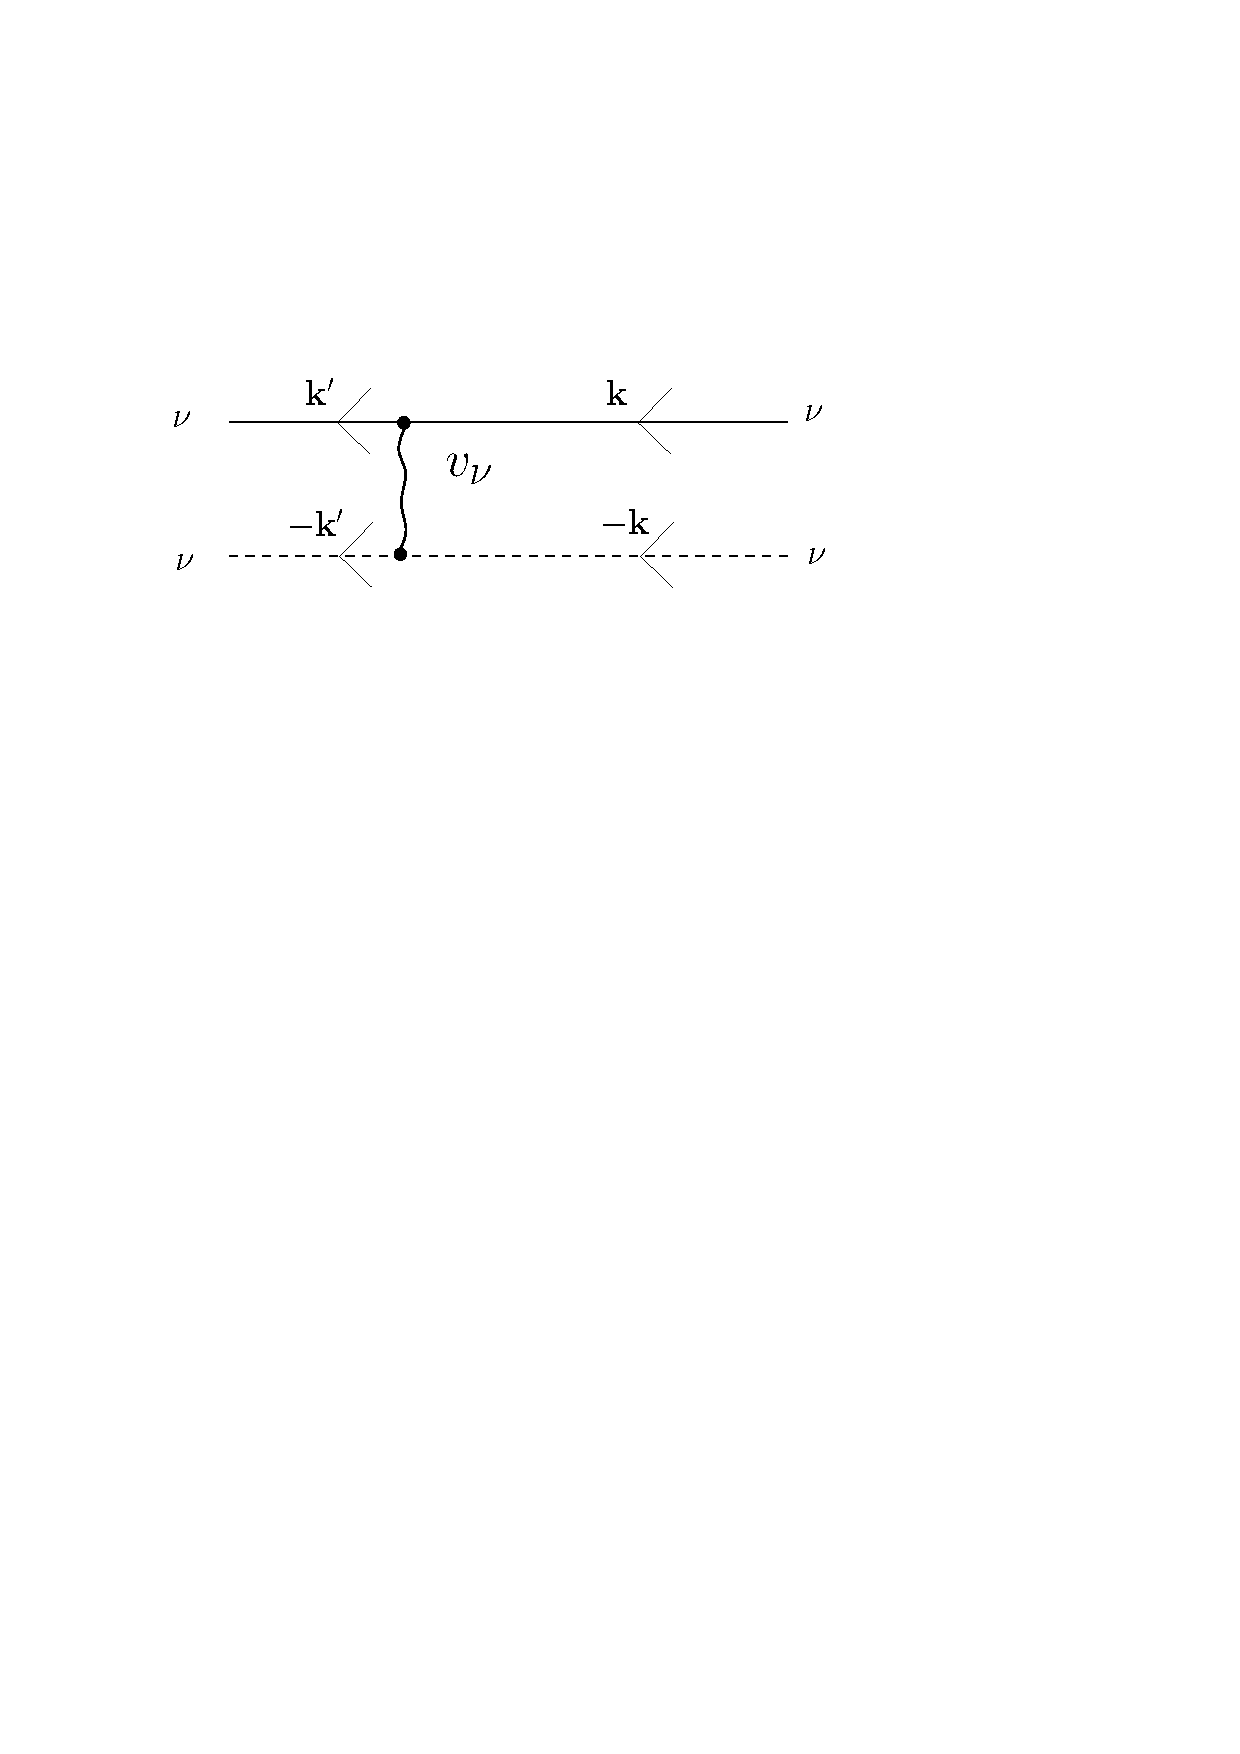
\includegraphics[width=.3\textwidth]{intraBand}}\quad
		\subfloat[Non-diagonal interaction]{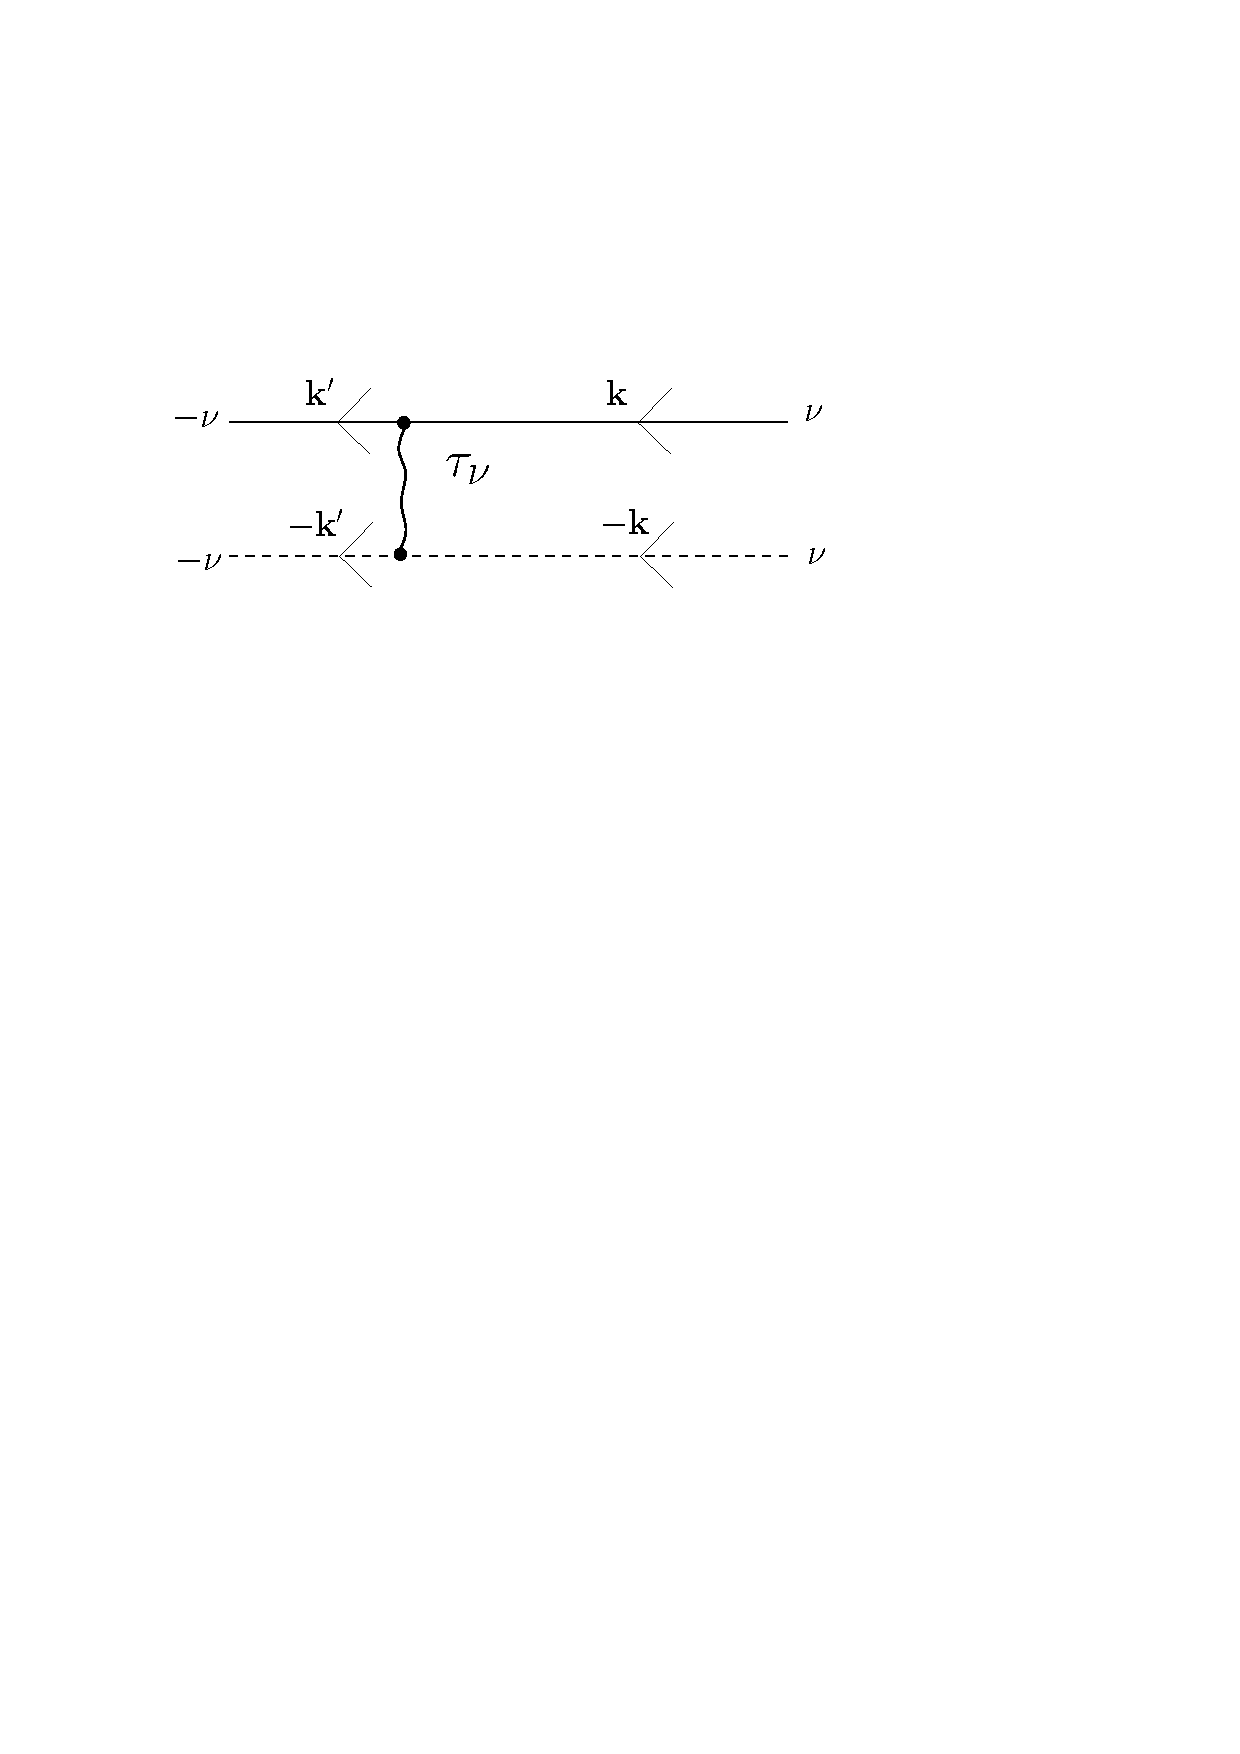
\includegraphics[width=.30\textwidth]{interBand}\label{fig:inter}}
	\caption{Diagonal and non-diagonal subband interaction without shared species}
\end{figure}
\item The second set of interaction potentials deal with pairs sharing a fermion $\alpha$ in subband $1$, namely $B^{\dg}_{\vk,1,1}$ and $B^{\dg}_{\vk,-1,-1}$. These fermion pairs interact through the diagonal processes of Fig. \ref{3intraBand} with a transfer scattering $\tau$, the fermion $\alpha$ now staying in the $\nu=1$ band.  All the other $V 
\left(\begin{smallmatrix}\nu_{\alpha}^{'}&\nu_{\alpha}^{}\\ \nu_{\beta}^{'}&\nu_{\beta}^{}\end{smallmatrix}\right)$ scatterings are taken equal to zero.  In this case, the $(-1)$ states of fermion $\alpha$ stay uncoupled and play no role in the problem.  When the number of fermions $\alpha$ and $\beta$ increases, a $B^{\dg}_{\vk,1,1}$ pair feels not only the other $B^{\dg}_{\vk,1,1}$ pairs by Pauli blocking, but it also feels the $B^{\dg}_{\vk,1,-1}$ pairs because $B^{\dg}_{\vk,1,1}$ and $B^{\dg}_{\vk,1,-1}$ share the same fermion operator $a^{\dg}_{\vk,1}$.
\begin{figure}[hhtb]
	\centering
	         \subfloat[Diagonal interaction]{\label{fig:3intra}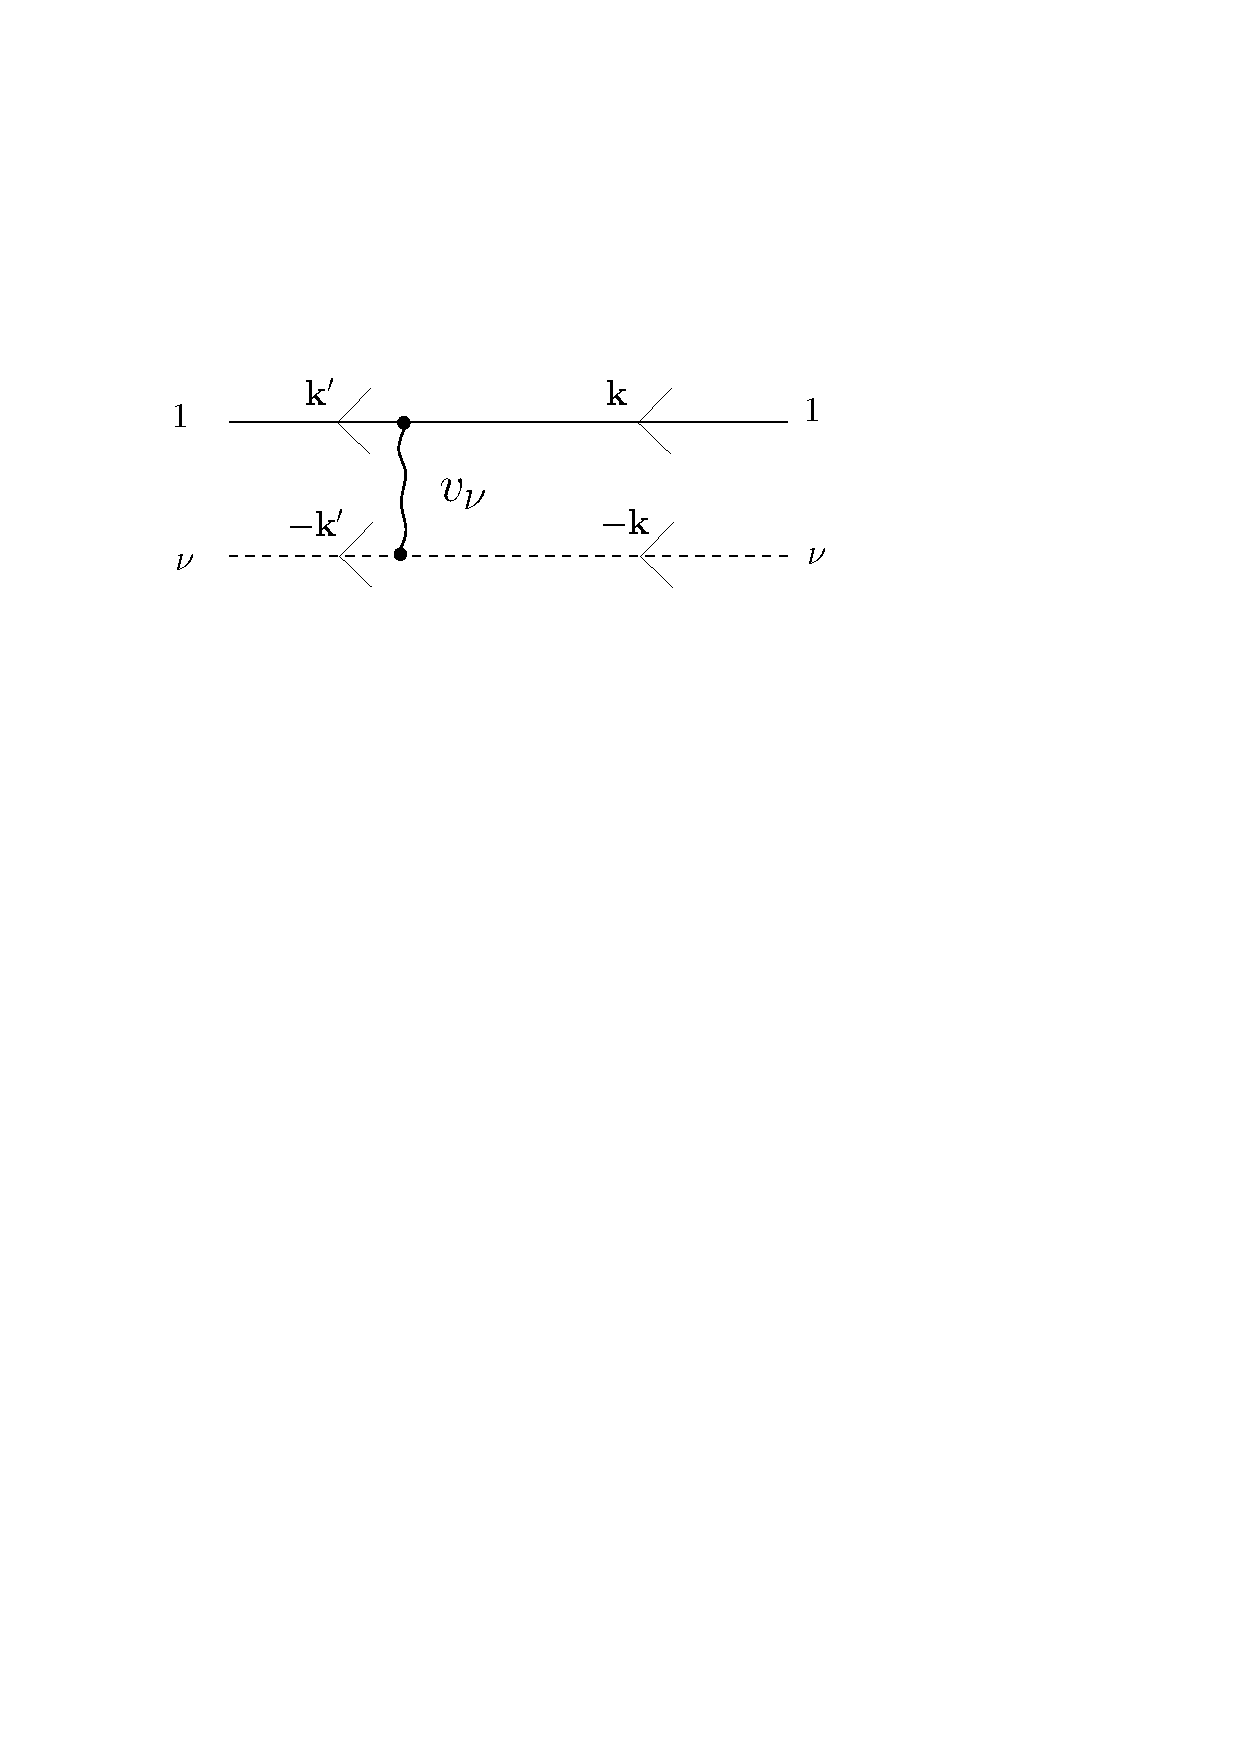
\includegraphics[width=.3\textwidth]{3intraBand}}\quad
		\subfloat[Non-diagonal interaction]{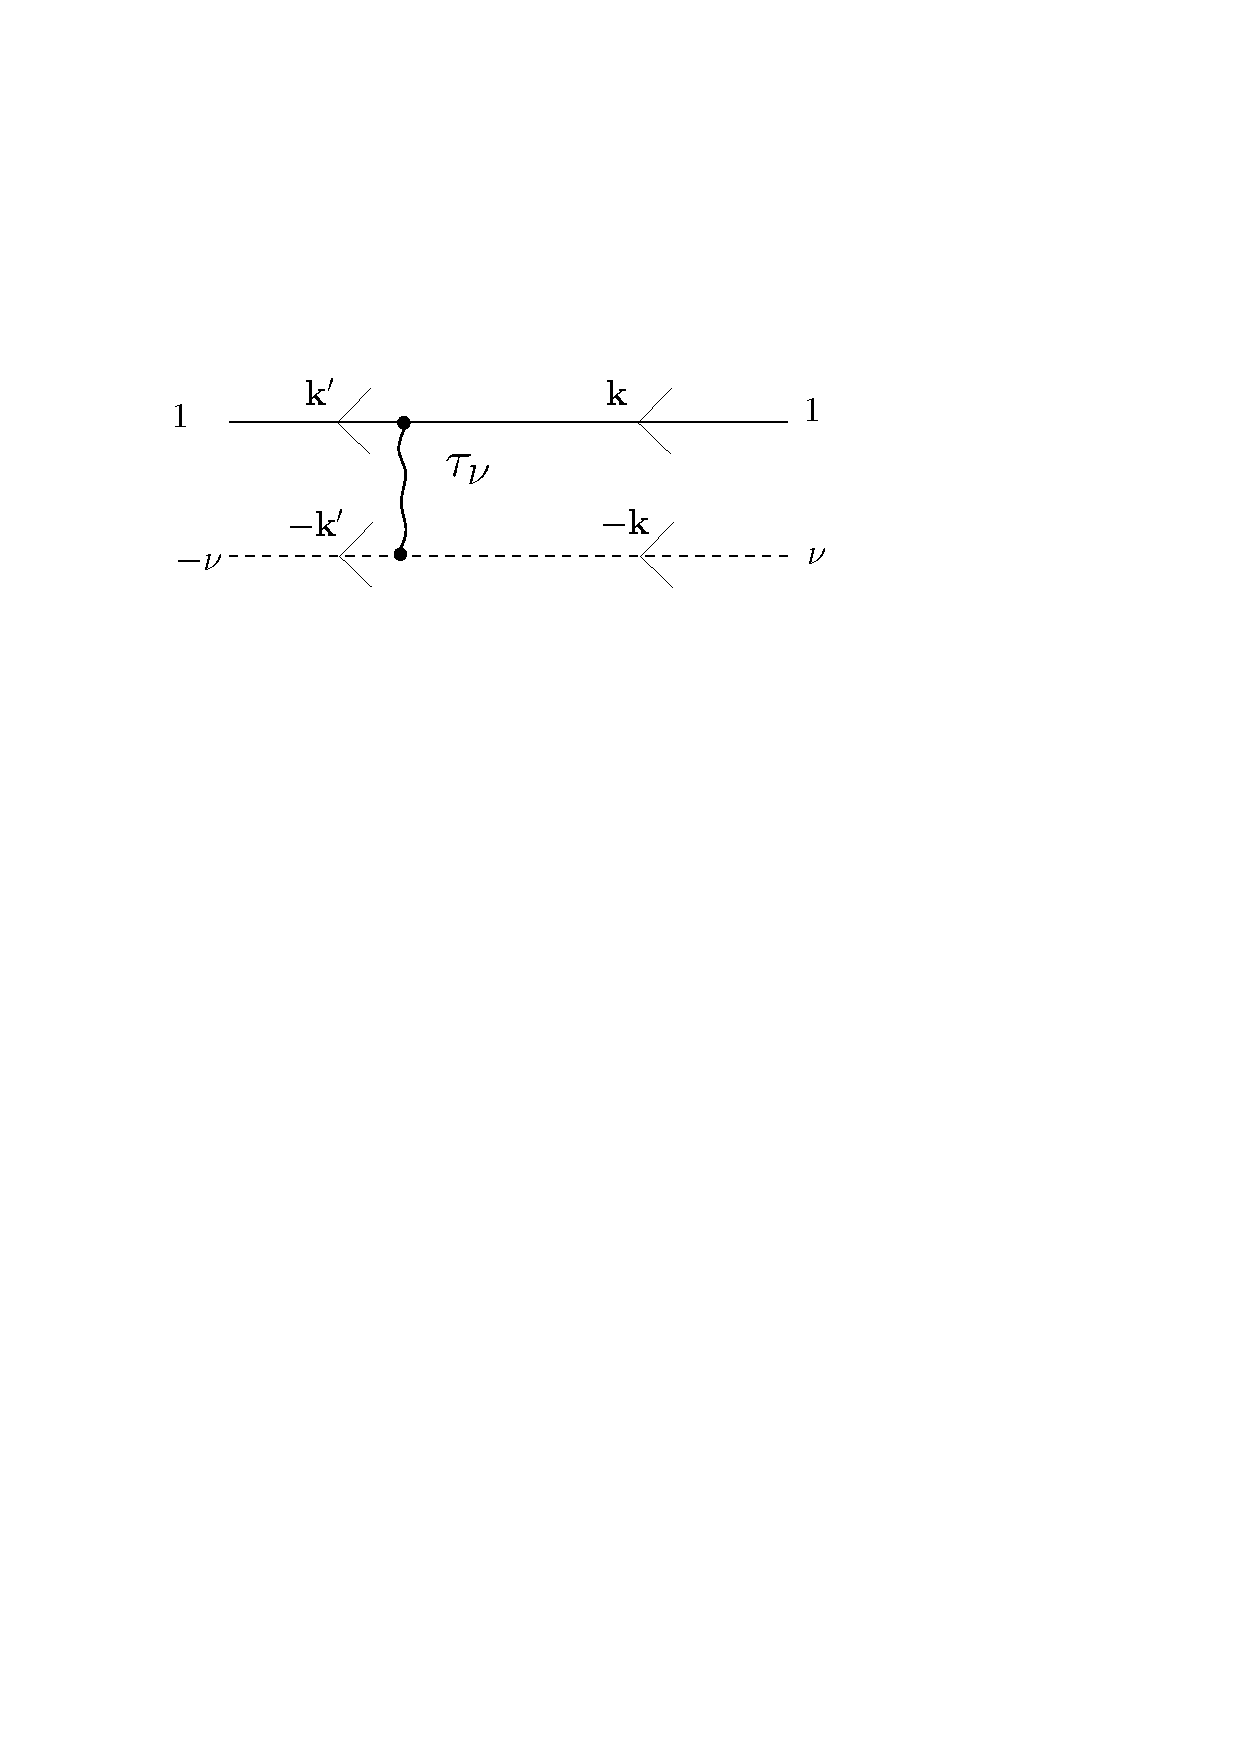
\includegraphics[width=.30\textwidth]{3interBand}\label{fig:3inter}}
	\caption{Diagonal and non-diagonal subband interaction with shared species}
\end{figure}
\end{enumerate}
\end{document}
